% ============================================================================
% Architectuur- en ontwikkelstrategie Invaarcalculator v3.9.2
% Geschikt voor pdfLaTeX. Documenteert IT-architectuur, ontwikkel-workflow
% en validatie-strategie op hoofdlijnen.
%
% Actualisatie van v3.0.158 (16 mei 2026). Belangrijkste wijzigingen sinds
% die versie: de basic/expert-variantsplitsing, de M3/RDR-module (Monte-
% Carlo in een Web Worker) + collectieve pool-engine, de leeftijdgebonden
% DNB-RTS-curve, de AOW-poort, de 5-delige restart-set met 00_START_HIER.md,
% de nieuwe versie-discipline (3.X.Y, per variant) en de gegroeide testgate
% (37 tests, 0 known-fail).
% ============================================================================

\documentclass[11pt,a4paper]{article}

\usepackage[utf8]{inputenc}
\usepackage[T1]{fontenc}
\usepackage[dutch]{babel}
\usepackage{lmodern}
\usepackage{microtype}

\usepackage[a4paper,margin=2.5cm]{geometry}
\usepackage{parskip}
\setlength{\parindent}{0pt}

\usepackage{amsmath}
\usepackage{amssymb}

\usepackage{booktabs}
\usepackage{longtable}
\usepackage{array}
\usepackage{tabularx}

\usepackage{enumitem}
\setlist[itemize]{leftmargin=*,topsep=2pt,itemsep=2pt}

\usepackage{textcomp}
\usepackage{fancyhdr}
\usepackage{lastpage}
\usepackage{datetime}
\usepackage{etoolbox}
\settimeformat{hhmmsstime}

\usepackage{titlesec}
\titleformat{\section}{\normalfont\Large\bfseries}{\thesection}{0.7em}{}
\titleformat{\subsection}{\normalfont\large\bfseries}{\thesubsection}{0.7em}{}

\newcommand{\code}[1]{\texttt{#1}}

\usepackage{xcolor}
\definecolor{linkblue}{HTML}{0B4F8B}
\definecolor{boxbg}{HTML}{F4F4F2}
\definecolor{boxborder}{HTML}{D0D0D0}

\usepackage{hyperref}
\hypersetup{colorlinks=true,linkcolor=linkblue,urlcolor=linkblue}

\usepackage{tikz}

\emergencystretch=1.5em

\title{%
  \textbf{Architectuur- en ontwikkelstrategie}\\[0.5em]
  \Large Invaarcalculator\texttrademark{}\ v3.9.2\\[0.3em]
  \normalsize IT-architectuur, workflow en validatie-strategie op hoofdlijnen
}
\author{Innovation Nestor}
\date{\today}

\begin{document}
\maketitle
\thispagestyle{empty}

\pagestyle{fancy}
\fancyhf{}
\fancyhead[L]{\small Invaarcalculator\texttrademark{} --- Architectuur \& workflow}
\fancyhead[R]{\small Innovation Nestor}
\fancyfoot[L]{\small Pagina \thepage{} van \pageref{LastPage}}
\fancyfoot[R]{\small v3.9.2 \ --- \ \today\ \currenttime}
\renewcommand{\headrulewidth}{0.4pt}
\renewcommand{\footrulewidth}{0.4pt}
\setlength{\headheight}{14pt}

\fancypagestyle{plain}{%
  \fancyhf{}%
  \fancyhead[L]{\small Invaarcalculator\texttrademark{} --- Architectuur \& workflow}%
  \fancyhead[R]{\small Innovation Nestor}%
  \fancyfoot[L]{\small Pagina \thepage{} van \pageref{LastPage}}%
  \fancyfoot[R]{\small v3.9.2 \ --- \ \today\ \currenttime}%
  \renewcommand{\headrulewidth}{0.4pt}%
  \renewcommand{\footrulewidth}{0.4pt}%
}

\vspace{1em}
\tableofcontents
\newpage

% ============================================================================
\section{Inleiding}

Dit document beschrijft op hoofdlijnen hoe de Invaarcalculator is opgebouwd en hoe hij wordt ontwikkeld. Het is geschreven voor lezers die de inhoudelijke onderwerpen (Modelspecificatie, Demografie-verantwoording, M3/RDR-specificatie) elders al kennen en willen begrijpen hoe het kale instrument er onder de motorkap uitziet --- welke technologieën gebruikt zijn, hoe nieuwe versies tot stand komen, hoe correctheid wordt geborgd, en hoe de samenwerking met AI-assistenten in de praktijk werkt.

Dit is een actualisatie van de versie van 16 mei 2026 (v3.0.158). De grootste verschuivingen sindsdien: de calculator bestaat nu in twee varianten (\emph{basic} en \emph{expert}) uit één codebase, de expert-variant bevat een Monte-Carlo-module voor de risicodelingsreserve (M3/RDR) die live in de browser rekent, en de sessie-overdracht en validatie zijn aanzienlijk verder geformaliseerd.

% ============================================================================
\section{Architectuur in één pagina}
\label{sec:overview}

\subsection{Wat de calculator is}

Twee zelfdragende HTML-bestanden, gebouwd uit één codebase: \code{basic} (ongeveer 0,4\,MB) en \code{expert} (ongeveer 17\,MB), draaiend in elke moderne browser. Geen server, geen database, geen backend. Alle berekeningen voltrekken zich in JavaScript in de browser van de gebruiker; er gaat geen invoer over het netwerk de deur uit.

In beide varianten zitten de AG2024-sterftafel en de leeftijdgebonden DNB-rentetermijnstructuur als JSON ingebed. De expert-variant bevat daarnaast een subset van 10.000 scenario's uit de DNB-scenarioset (P-set) plus de RDR-rekenworker --- vandaar het grootteverschil. De Modelspecificatie en de Demografie-verantwoording zitten, anders dan in eerdere versies, \emph{niet} meer als PDF in het HTML-bestand ingebed; de documentatie staat als LaTeX-bron en PDF in de repository.

\subsection{Twee varianten: basic en expert}
\label{sec:varianten}

Sinds de variant-splitsing levert dezelfde codebase twee producten:

\begin{itemize}
\item \textbf{Basic} --- gratis variant voor deelnemers. Een wizard (triage $\rightarrow$ persoonlijke gegevens $\rightarrow$ financieel $\rightarrow$ resultaat) zonder technische sliders; de rekenrente is een vaste, leeftijdgebonden DNB-RTS-waarde. Een AOW-poort wijst geboortedata af waarvoor de AOW-leeftijd nog niet bereikt is (een ander uitkeringsregime dat de motor niet waardeert). Het resultaatscherm toont naast het hoofdresultaat een dekkingsgraad$\times$projectierente-gevoeligheidsmatrix.
\item \textbf{Expert} --- variant voor bestuur, helpdesk en audit. Alle parameters instelbaar (discontovoet, dekkingsgraad, bijstort, projectierente), met daarbovenop het M3/RDR-paneel (uitkeringswaaier P10/P50/P90), een fonds-brede collectieve pool-weergave en aanvullende grafieken.
\end{itemize}

De splitsing is een build-as, geen tweede codebase. De build-flag \code{--variant=basic|expert} stuurt esbuild-aliassen (\code{\textasciitilde variant}, \code{\textasciitilde m2}, \code{\textasciitilde m3}, \code{\textasciitilde help}) die per variant óf de echte module óf een lege stub inbundelen. De basic-bundel bevat zo geen expert-bytes: geen M3-paneel, geen scenario-data, geen worker. Beide varianten hebben een eigen versieteller (zie \S\ref{sec:versie}); op het moment van schrijven basic 3.9.2 en expert 3.7.0.

\subsection{Distributie}

De broncode staat publiek op GitHub (\href{https://github.com/Invaarcalculator/invaarcalculator.git}{github.com/Invaarcalculator/invaarcalculator}). De build schrijft naast de versie-gestempelde bestanden ook \code{index.html} (kopie van basic) en \code{expert.html} (kopie van expert); GitHub Pages serveert die statisch op \href{https://invaarcalculator.nl}{invaarcalculator.nl} respectievelijk \href{https://invaarcalculator.nl/expert.html}{invaarcalculator.nl/expert.html}. Geen CI/CD-pipeline; geen automatische deployment; updates gebeuren door drag-and-drop van de bestanden in de GitHub-webinterface.

\subsection{Componenten}

\begin{figure}[h]
\centering
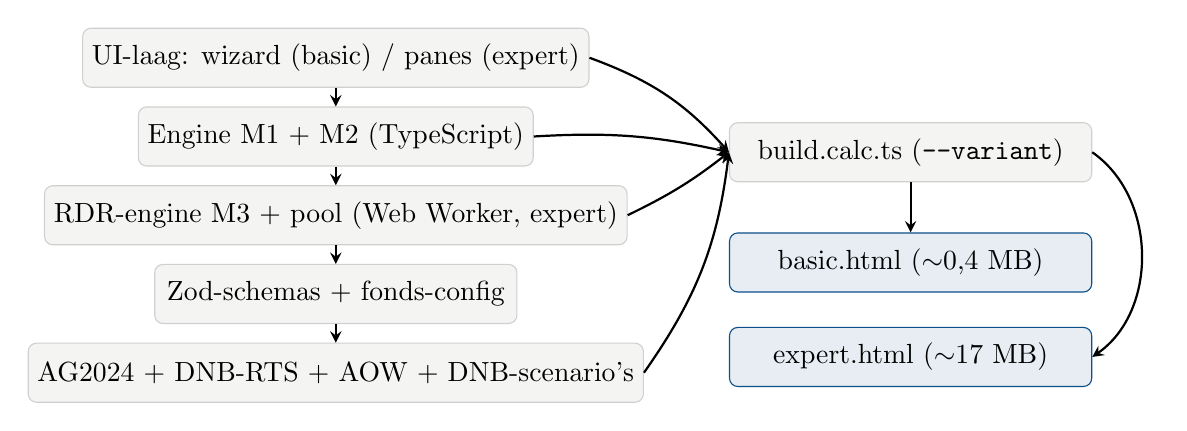
\begin{tikzpicture}[node distance=0.8cm,
                    box/.style={draw,rounded corners=3pt,minimum width=4.6cm,minimum height=0.75cm,fill=boxbg,draw=boxborder},
                    edge/.style={->,thick,>=stealth}]
  \node[box] (ui) at (0,5.0) {UI-laag: wizard (basic) / panes (expert)};
  \node[box] (engine) at (0,4.0) {Engine M1 + M2 (TypeScript)};
  \node[box] (rdr) at (0,3.0) {RDR-engine M3 + pool (Web Worker, expert)};
  \node[box] (schema) at (0,2.0) {Zod-schemas + fonds-config};
  \node[box] (data) at (0,1.0) {AG2024 + DNB-RTS + AOW + DNB-scenario's};
  \node[box] (build) at (7.3,3.8) {build.calc.ts (\code{-{}-variant})};
  \node[box,fill=linkblue!10,draw=linkblue] (outb) at (7.3,2.4) {basic.html ($\sim$0,4 MB)};
  \node[box,fill=linkblue!10,draw=linkblue] (oute) at (7.3,1.2) {expert.html ($\sim$17 MB)};

  \draw[edge] (ui) -- (engine);
  \draw[edge] (engine) -- (rdr);
  \draw[edge] (rdr) -- (schema);
  \draw[edge] (schema) -- (data);
  \draw[edge] (ui.east) to[bend left=14] (build.west);
  \draw[edge] (engine.east) to[bend left=8] (build.west);
  \draw[edge] (rdr.east) to[bend right=6] (build.west);
  \draw[edge] (data.east) to[bend right=14] (build.west);
  \draw[edge] (build) -- (outb);
  \draw[edge] (build.east) to[bend left=55] (oute.east);
\end{tikzpicture}
\caption{Component-overzicht. De engine-lagen voeren berekeningen uit; de UI-laag rendert resultaten; de schema-laag valideert de fonds-parameters; de bundler combineert alles per variant tot één bestand. De RDR-laag en de scenario-data gaan alleen mee in de expert-build.}
\end{figure}

% ============================================================================
\section{Technologie-keuzes}
\label{sec:tech}

\subsection{TypeScript voor engine en UI}

De gehele rekenkern, UI-rendering en build-tooling zijn in TypeScript geschreven. Reden: één taal voor alle code-paden, statisch type-systeem voor compile-time-fouten, en herbruikbaarheid tussen browser-runtime en server-side (Node.js) test-runner. De code is geschreven zonder framework: vanilla DOM-manipulatie, geen React/Vue/Svelte. Ook bij de huidige omvang (ongeveer 23.600 regels TypeScript, waarvan de UI-orchestratie in \code{src/ui.app.ts} alleen al ruim 4.200 regels) blijft die keuze houdbaar: de render-loop is één functie, state is één object, en er is geen build-afhankelijkheid van een framework-ecosysteem.

\subsection{Zod voor schema-validatie}

Alle fonds-parameters worden geladen via Zod-schemas. Dat geeft compile-time TypeScript-types \emph{en} runtime-validatie van de invoer. Bij ongeldige fonds-configuratie faalt de calculator hard bij het laden, niet stilletjes bij een rekenstap. Het schema-bestand (\code{src/schema.v2.ts}) is ruim 1.100 regels lang en bevat per veld de bronvermelding en de toegestane waarde-range.

\subsection{esbuild voor bundeling}

De build-stap (\code{build.calc.ts}) gebruikt esbuild om alle TypeScript-bestanden in \'e\'en JavaScript-bundel te compileren, voegt de embedded data toe (AG2024-sterftafel, DNB-RTS; voor expert ook de scenario-subset), en wraps alles in een HTML-template met inline CSS. De variant-keuze loopt via esbuild-aliassen (\S\ref{sec:varianten}). Voor de expert-build draait een tweede esbuild-pass die de RDR-worker als zelfstandige IIFE-string bundelt; die string wordt in de HTML gebakken en pas in de browser via een \code{Blob}-URL tot Worker gemaakt --- zo blijft de single-file-deploy intact, zonder los \code{.js}-bestand. Resultaat: per variant één zelfdragend HTML-artefact.

\subsection{Web Worker voor de M3/RDR-module}

Het M3-paneel (expert) draait een Monte-Carlo-projectie van de risicodelingsreserve live in de browser, in een Web Worker --- buiten de UI-thread, zodat de pagina responsief blijft. De waaier rekent live op 1.000 scenario's uit de embedded subset van 10.000 (visueel gelijkwaardige P10/P50/P90-banden tegen een fractie van de rekentijd); herberekening gebeurt automatisch en gedebounced bij elke invoerwijziging. Dezelfde worker bedient ook de collectieve pool-modus (fonds-brede reserve-projectie); de berichten zijn getagd zodat waaier- en pool-resultaten elkaar niet kunnen verwarren.

\subsection{pdfLaTeX voor documenten}

De Modelspecificatie, de Demografie-verantwoording, de M3/RDR-specificatie en dit document zelf zijn pdfLaTeX-bronnen, gecompileerd naar PDF. Ze staan als plaintext-bron plus PDF in de repository; ze worden niet meer in het HTML-bestand ingebed. Reden voor LaTeX: typografische kwaliteit voor formele documentatie, en plaintext-bron die in versiebeheer kan zonder binary-diff-problemen.

\subsection{Geen externe dependencies in productie}

De gebouwde HTML-bestanden bevatten geen externe scripts, fonts, of API-aanroepen. Geen Google Fonts, geen jQuery-CDN, geen externe icoon-bibliotheek. Devtime-dependencies (TypeScript, Zod, jsdom voor tests, esbuild, tsx) zijn allemaal beperkt tot build- en test-fasen; in de gebruiker-zichtbare HTML zit alleen wat de gebruiker nodig heeft om de calculator te draaien.

\subsection{Geen tracking, geen ads, geen cookies}

De pagina zet geen cookies, gebruikt geen analytics, en stuurt geen invoer naar een server. De enige netwerk-activiteit is het \'e\'enmaal ophalen van het HTML-bestand bij paginaload via GitHub Pages. Wat GitHub Pages aan eigen logging doet (IP-adres, User-Agent, tijdstempel) staat buiten de invloed van deze tool en is gedocumenteerd in de privacy-sectie van de UI.

% ============================================================================
\section{Codebase-structuur}
\label{sec:codebase}

\begin{longtable}{@{}>{\raggedright\arraybackslash}p{0.34\textwidth}>{\raggedright\arraybackslash}p{0.60\textwidth}@{}}
\toprule
\textbf{Pad} & \textbf{Inhoud} \\
\midrule
\endhead
\code{src/engine.m1.ts} & Kapitaalwaarde-berekening van de huidige aanspraak (KV), inclusief AG2024-sterftafel-lookups, annu\"iteitsfactoren, en joint-life-partner-mechaniek met broken-heart-correctie. \\
\code{src/engine.m2.ts} & Persoonlijk pensioenvermogen na invaren (PPV), inclusief fondsbalans-decompositie, cohort-aggregatie voor de fondsschalingsfactor $x_{\text{fonds}}$, en de alternatieve invaarmethode (Ortec-proxy). \\
\code{src/rdr/} & M3/RDR-module: \code{engine.rdr.ts} (individuele RDR-projectie, Monte-Carlo over de DNB-scenario's), \code{pool.rdr.ts} (collectieve fonds-brede reserve-pool), \code{rdr.worker.ts} (Web-Worker-entry), plus smoothing, scenario-subset-logica en de normatieve modulespecificatie \code{SPECIFICATIE\_M3\_RDR\_v0.3.tex}/\code{.pdf}. \\
\code{src/schema.v2.ts} & Zod-schemas voor fonds-parameters en deelnemer-input; runtime-validatie met inline bronvermelding per veld. \\
\code{src/dnbrts.ts} & Leeftijdgebonden lookup op de embedded DNB-rentetermijnstructuur (curve in plaats van een vlakke scalar). \\
\code{src/belasting.ts} & Bruto/netto-conversie voor de netto-invoerroute in basic. \\
\code{src/ui.app.ts} & UI-orchestratie: state-management, event-handlers, modal-orchestratie, render-loop, de basic-wizard inclusief AOW-poort en resultaatscherm. \\
\code{src/ui.m2.ts}, \code{src/ui.m3.ts} (+\,\code{.stub.ts}) & Expert-panes per rekenmodule (sliders, KPI-blokken, M3-waaier- en pool-pane). De \code{.stub.ts}-tegenhangers zijn lege drop-ins voor de basic-build. \\
\code{src/ui.modal.ts}, \code{src/ui.toast.ts}, \code{src/ui.shared.ts} & Accessibility-correcte modal-helper, niet-blokkerende toast-meldingen, gedeelde UI-hulpfuncties. \\
\code{src/variant.config.ts} (+\,\code{variant.basic.ts}, \code{variant.expert.ts}) & Variant-definities: per-variant versieteller, feature-vlaggen, variant-specifieke teksten, plus de changelog per variant als commentaar. \\
\code{src/content/help/*.ts} & Tekstuele helpinhoud per parameter, gescheiden van rekencode; aparte registers voor basic en expert. \\
\code{fondsen/sspf/} & SSPF-specifieke parameter-waarden (fondsvermogen, dekkingsgraad, demografie), de Bijlage-B-ervaringssterftetabel en de worst-case-cohortmix voor de fondsmix-band. \\
\code{data/} & Externe bron-data: de DNB-RTS-CSV en het SVB-schema geboortemaand$\rightarrow$AOW-leeftijd (basis van de AOW-poort). \\
\code{rdr\_run/} & DNB-scenariosets en de herbouw-pijplijn voor de CLI-toets van de RDR-engine. \\
\code{fixtures/}\allowbreak\code{golden\_sspf\_default.json} & Vastgepinde anker-uitkomsten voor regressie-detectie. \\
\code{scripts/run-tests.ts} & Test-runner met manifest-gestuurde uitvoering en pass/fail/known-fail-categorisatie. \\
\code{scripts/snapshot.ts} & Sessie-afsluitings-tool: test, bouwt beide varianten, zipt de codebase, bundelt en verifieert de restart-set. \\
\code{build.calc.ts} & Bundle-script: combineert TypeScript-bundel en embedded data per variant in \'e\'en HTML. \\
\bottomrule
\end{longtable}

Totale codebase: ongeveer 23.600 regels TypeScript verdeeld over deze bestanden. De M1+M2-engine is ongeveer 85\,KB; de RDR-laag (individuele engine + pool) komt daar met ongeveer 34\,KB bovenop.

\subsection{Scheiding engine en UI}

Een bewuste discipline: rekencode en UI-code raken elkaar niet. De engine-bestanden (\code{engine.m1.ts}, \code{engine.m2.ts}, \code{engine.rdr.ts}, \code{pool.rdr.ts}) zijn pure functies --- gegeven dezelfde input leveren ze dezelfde output, zonder DOM-afhankelijkheden, zonder side-effects. De UI-laag bouwt input-objecten op uit DOM-events, roept de engine aan, en rendert het resultaat; de RDR-worker is daartussen een dunne transportlaag. Deze scheiding maakt dat de engines los van een browser getest kunnen worden (engine-tier-tests in Node.js, plus een CLI-toets van de RDR-engine tegen dezelfde scenarioset als het paneel) en dat de UI-laag onafhankelijk gewijzigd kan worden (jsdom-tier-tests).

% ============================================================================
\section{Ontwikkel-workflow}
\label{sec:workflow}

\subsection{Sessies als ontwikkelingseenheid}

Het werk gebeurt in afgeronde sessies van enkele uren tot enkele dagen. Een sessie begint met het uploaden van de \emph{restart-set} uit de voorgaande sessie --- vijf bestanden, ook gebundeld beschikbaar als \code{restart-set\_v\textless X.Y.Z\textgreater.zip}:

\begin{itemize}
\item \code{Keep-14\_v\textless X.Y.Z\textgreater\_sessie.zip} --- volledige werkdirectory-snapshot
\item \code{00\_START\_HIER.md} --- het startdocument: sessiegeschiedenis, openstaande punten en de vaste opstart- en afsluitprocedure
\item \code{HANDOFF\_v\textless X.Y.Z\textgreater.md} --- wat er gewijzigd is, welke validatie gedaan is, openstaande items
\item \code{calculator\_v\textless X.Y.Z\textgreater\_basic.html} en \code{calculator\_v\textless X.Y.Z\textgreater\_expert.html} --- de gebouwde varianten voor visuele referentie
\end{itemize}

Een sessie eindigt met dezelfde set voor de nieuwe versie. De handoff is altijd leidend voor de actuele status; \code{00\_START\_HIER.md} houdt de keten van sessies vast en de zip bevat alle historische handoffs als referentie. Deze procedure bestaat omdat eerdere sessie-overgangen bij herhaling iets lieten vallen; het snapshot-script (\S\ref{sec:handoff}) dwingt haar inmiddels machinaal af.

\subsection{De handoff-discipline}
\label{sec:handoff}

Elke versie krijgt een eigen handoff-document met daarin:

\begin{itemize}
\item Wat is gewijzigd (welke bestanden, welke functies, welke gedragsverandering)
\item Welke validatie is gedaan (test-resultaten, jsdom-verificatie, eventuele numerieke vergelijking)
\item Open punten of vervolg-aanbevelingen
\item Versie-bump-spoor: \code{src/variant.config.ts} (per-variant \code{version}), \code{package.json} \code{version}, en --- bij engine-wijzigingen --- \code{fixtures/}\allowbreak\code{golden\_sspf\_default.json} \code{release\_anchor}
\end{itemize}

Het snapshot-script faalt hard als de bijbehorende handoff ontbreekt, en verifieert na het bundelen dat de uitgepakte restart-set exact overeenkomt met de set die \code{00\_START\_HIER.md} voorschrijft --- niet meer, niet minder. Dat is bewust: een versie zonder handoff is niet vindbaar bij toekomstige sessies, en zou de continu\"iteit van de samenwerking met AI-assistenten breken.

\subsection{Versie-discipline}
\label{sec:versie}

\begin{longtable}{@{}>{\raggedright\arraybackslash}p{0.44\textwidth}>{\raggedright\arraybackslash}p{0.22\textwidth}>{\raggedright\arraybackslash}p{0.28\textwidth}@{}}
\toprule
\textbf{Soort wijziging} & \textbf{Versie-bump} & \textbf{Handoff-naam} \\
\midrule
\endhead
Variant-specifiek (UI, teksten, resultaatscherm) & Alleen de geraakte variant & \code{HANDOFF\_v\textless X.Y.Z\textgreater.md} \\
Gedeelde lagen (engine, fondsconfig, gedeelde content) & Beide varianten & \code{HANDOFF\_v\textless X.Y.Z\textgreater.md} \\
Tooling (scripts, tests, docs) & Nee & \code{HANDOFF\_v\textless X.Y.Z\textgreater}\allowbreak\code{-tooling.md} \\
\bottomrule
\end{longtable}

Versie-nummers volgen het patroon \code{3.X.Y}: een minor-bump per inhoudelijke ronde, een patch-bump voor vervolgrondes binnen hetzelfde thema. (Tot en met v3.0.251 telde het patch-nummer simpelweg sessies; sinds v3.1.0 dragen minor-bumps betekenis.) Sinds de variant-splitsing heeft elke variant een eigen teller in \code{variant.config.ts}, met de changelog als commentaar bij die teller. De tellers mogen divergeren: een reeks basic-only rondes laat expert staan --- op het moment van schrijven basic 3.9.2 tegenover expert 3.7.0. Bij gedeelde wijzigingen bumpen beide. De codebase-zip en de restart-set dragen de hoogste van de twee.

% ============================================================================
\section{Validatie-strategie}
\label{sec:validatie}

\subsection{Test-suite}

Bij elke sessie-afsluiting draait een volledige test-run (\code{npm run test:all}). Het manifest in \code{scripts/run-tests.ts} stuurt op dit moment 37 tests in twee tiers:

\begin{itemize}
\item \textbf{Engine-tier} (19 tests): pure TypeScript-tests draaiend in Node.js, geen browser nodig. Onder andere KV-smoke-tests, M2-cascade-tests, alternatieve-methode-consistentie, de M3-doorgifte- en grondslag-tests, de RDR-engine-, smoothing- en scenario-tests, een typecheck-guard, build-portability en de \emph{golden-fixture-test} (zie hieronder).
\item \textbf{Jsdom-tier} (18 tests): tests die de gebouwde HTML in een gesimuleerde browser laden en interactief gedrag verifi\"eren --- end-to-end-berekening, komma-invoer, modal-toegankelijkheid, toast-gedrag, extensie-noise-filter, mobiele layout, typografie en dynamic type, de AOW-poort, de hoog/laag-volgorde, het parameter-scherm, en een parity-test tussen basic en expert.
\end{itemize}

Het manifest kent naast ``pass'' de categorie ``known-fail'' (bekend rood, telt niet als blokkade; een known-fail die \emph{slaagt} wordt juist gemeld als kandidaat voor promotie). Op dit moment staat de gate op 37 ``pass'' en 0 ``known-fail''. Een rode uitslag op een pass-test blokkeert de sessie-afsluiting: het snapshot-script weigert dan een restart-set te produceren.

\subsection{Golden-fixture}

Het bestand \code{fixtures/}\allowbreak\code{golden\_sspf\_default.json} bevat de exacte verwachte engine-uitkomst voor het UI-default-scenario (70-jarige man, EUR 100.000 pensioen, geen partner, SSPF-defaults). Bij elke engine-wijziging wordt deze fixture gecontroleerd: een afwijking van meer dan een fractie van een procent op KV, PPV of intermediate-grootheden vereist een expliciete update van het fixture-bestand mét bevestiging van de nieuwe ``ankerwaarde''. Ook een bewuste data-update (zoals het verwerken van nieuwe jaarverslag-cijfers in de fondsconfig) loopt langs deze route: de fixture wordt dan herijkt en de herijking wordt in de handoff verantwoord.

Dit beschermt tegen drift: kleine code-wijzigingen die per ongeluk een numerieke output verschuiven, slaan stuk op de golden-fixture-test en moeten dan verantwoord worden in de handoff voordat de fixture wordt geactualiseerd.

\subsection{Behavior-freeze voor refactors}

Bij refactor-stappen (opschoning, herstructurering, dode-code-verwijdering) gebruiken we een zwaardere check: de gebundelde JavaScript-output wordt per variant byte-voor-byte vergeleken met de vorige versie. Identiek (op de versie-string na) = bewezen geen gedragsverandering. Een refactor die de bundel-bytes onveranderd laat, is per definitie gedrag-neutraal en kan zonder verdere numerieke verificatie aanvaard worden.

\subsection{Parity basic--expert}

De engines van basic en expert zijn identiek; de varianten verschillen in UI en in default-keuzes (basic rekent op de vaste leeftijdgebonden DNB-RTS-waarde, expert laat de discontovoet instellen). Een geautomatiseerde parity-test in de jsdom-tier bewaakt dat beide builds bij gelijke invoer dezelfde kernuitkomsten geven, zodat de variant-splitsing een presentatie-laag blijft en geen rekenverschil kan worden. Daarnaast wordt bij variant-specifieke rondes via jsdom geverifieerd dat de niet-geraakte variant ook werkelijk ongewijzigde zichtbare output heeft.

\subsection{Jsdom-handmatige checks}

Voor UI-wijzigingen die de normale test-suite niet exhaustief dekt (nieuwe knoppen, modal-volgorde, dropdown-gedrag, het resultaatscherm), schrijven we per sessie ad-hoc jsdom-scripts die de gebouwde HTML laden en de specifieke wijziging verifi\"eren. Deze scripts staan niet in versie-controle --- ze zijn wegwerp-instrumenten voor \'e\'enmalige verificatie en worden in de handoff genoteerd onder ``Verificatie''. De keuze wat w\'el een geregistreerde test wordt, is bewust terughoudend: tests pinnen gedrag vast, en teksten of layout die nog itereren met de auteur worden niet voortijdig vastgepind.

\subsection{CLI-toets van de RDR-engine}

De RDR-engine kan buiten de browser worden gedraaid op de volledige DNB-scenarioset (pijplijn in \code{rdr\_run/}). Het M3-paneel is bij oplevering geverifieerd tegen die CLI-route (parity tussen paneel-uitkomsten en CLI-uitkomsten op dezelfde scenario-subset), zodat de browser-integratie --- worker, subset, doorwerking M1$\rightarrow$M2$\rightarrow$M3 --- geen eigen rekenwerkelijkheid kan ontwikkelen.

% ============================================================================
\section{Samenwerking met AI-assistenten}
\label{sec:ai}

\subsection{Wat AI-assistenten doen}

De codebase is iteratief tot stand gekomen in dialoog met meerdere AI-assistenten: voornamelijk Anthropic Claude (diverse versies, op het moment van schrijven Claude Fable 5) voor TypeScript-implementatie, modelspecificatie-redactie en architectuurkeuzes; PensioenGPT voor domeinspecifieke navigatie van Pensioenwet en bijlagen; aanvullende assistenten voor kruiscontrole en onderzoeksvragen.

\subsection{Waarom dit werkt}

Drie ontwerpkeuzes maken de samenwerking met AI-assistenten praktisch beheersbaar:

\begin{itemize}
\item \textbf{Pure functies in de engine}. Engine-code zonder side-effects is testbaar en reviewbaar zonder uitvoer-context; een AI-assistent kan een functie lezen, een test schrijven en de uitkomst beredeneren, allemaal op tekst-niveau.
\item \textbf{Zware schema-validatie}. Zod-fouten zijn expliciet en bevatten de context (welk veld, welke regel, welke waarde). Een AI-assistent die per ongeluk een verkeerd type-veld opstelt, krijgt direct een leesbare foutmelding terug die in de volgende iteratie de fix oplevert.
\item \textbf{Handoff-conventie}. Elke sessie sluit af met een handoff die de volgende sessie heropent zonder context-verlies, met \code{00\_START\_HIER.md} als vaste ingang. De handoff is leesbaar voor zowel mens als AI-assistent --- ze beschrijft niet alleen \emph{wat} gewijzigd is maar ook \emph{waarom}, zodat de volgende iteratie niet opnieuw door dezelfde argumenten hoeft.
\end{itemize}

\subsection{Wat de mens doet}

De rolverdeling in een sessie: de gebruiker (auteur) bepaalt richting en doel --- welk probleem, welke prioriteit, welke compromissen acceptabel zijn. De AI-assistent implementeert, test en verifieert, met de gebruiker als reviewer en eindbeslisser. Bij elke substanti\"ele keuze (architectuur, terminologie, modelaanname) levert de AI-assistent meerdere opties met afwegingen; de gebruiker selecteert.

\subsection{Wat dit niet is}

De AI-assistenten zijn geen autonomous-agents die zelf code committen. Elke wijziging gaat door dezelfde sessie-cyclus: handoff lezen, wijziging voorstellen, code maken, tests draaien, verificatie tonen, handoff schrijven, snapshot leveren. De gebruiker downloadt de restart-set en kiest of hij publiceert door \code{index.html} en \code{expert.html} in GitHub te plaatsen.

Aan de tool kunnen geen rechten worden ontleend; de inhoudelijke verantwoordelijkheid voor wat erin staat ligt bij de auteur, niet bij de AI-assistenten. Aanwezigheid van fouten --- in interpretatie van de Pensioenwet, in actuari\"ele formules, in code, of in numerieke uitkomsten --- kan niet worden uitgesloten en is op een aantal punten statistisch waarschijnlijk.

% ============================================================================
\section{Open-source en licentie}
\label{sec:opensource}

De volledige broncode is publiek beschikbaar onder CC BY-NC 4.0 (Creative Commons Naamsvermelding-Niet\-Commercieel 4.0 Internationaal). Dat betekent dat onafhankelijke verificatie van de berekeningen mogelijk is, dat afgeleide werken zijn toegestaan met bronvermelding, en dat commercieel gebruik expliciete toestemming vereist.

De documentatie (Modelspecificatie, Demografie-verantwoording, M3/RDR-specificatie, dit document) valt onder dezelfde licentie. Alle bronnen zijn als plaintext LaTeX in de codebase aanwezig zodat correcties zichtbaar zijn in versie-controle en niet in een binary-format zitten.

% ============================================================================
\section{Wat dit document niet beschrijft}

\begin{itemize}
\item \textbf{De rekenformules zelf}. Die staan in de Modelspecificatie; de M3/RDR-module heeft een eigen normatieve specificatie (\code{SPECIFICATIE\_M3\_RDR\_v0.3} in \code{src/rdr/}). Dit document beschrijft alleen de \emph{infrastructuur} eromheen.
\item \textbf{De cohort-data}. Bron, aging-methodiek en M/V-uitsplitsing van de SSPF-cohortbezetting staan in de Demografie-verantwoording.
\item \textbf{Specifieke implementatie-details}. Voor architectuur op functie-niveau: zie de inline-commentaar in de TypeScript-bestanden zelf en het bestand \code{ENGINE\_SPECIFICATIE\_v1.md} in de codebase (normatief specificatie-document, niet primair gebruikersgericht).
\item \textbf{Roadmap of geplande wijzigingen}. Per-sessie-status staat in de meest recente handoff en in \code{00\_START\_HIER.md}; een centrale roadmap-tracker bestaat niet.
\end{itemize}

\vspace{2em}
\hrule
\vspace{0.5em}
\emph{Einde architectuur- en ontwikkelstrategie.}

\end{document}
